\subsection{Overview}
\label{sec:migration-protocol}
\label{sec:log-entries}

During migration a set of slots is being moved from a donor shard group to a recipient shard group.
A coordinator $C$ splits the slots into \emph{migration groups} $G_1, \dots, G_n$ and instructs the donor leader to migrate them to the recipient leader. 
Groups are moved in the form of a transaction, by the \emph{Migration Manager (MM)} (a dedicated thread that controls the migration) of each leader.
Each group $G_i = \{s_1, \dots, s_m\}$ is a set of slots, and each slot $s_j$ contains the keys that map to it (e.g., by hashing), together with their values.
The key-value pairs of a slot are stored in blocks of SAMM allocator that the slot owns (Section~\ref{sec:samm}).
Migrating $G_i$ means transferring the blocks of its slots belonging to $G_i$.
Blocks are being moved as bulk, using one-sided RDMA, and never go through the log.
During migration, only decisions related to migration that must survive a crash are appended to each shard group's replicated log.
Under the fault model of Section~\ref{sec:fault-model}, our protocol ensures that
(i)~committed writes are never lost,
(ii)~a read never returns data that is only partially migrated or not yet replicated, and
(iii)~once a migration starts, it always runs to completion and is never rolled back.
Properties (i) and (ii) come from Fulva~\cite{fulva}.
The protocol has a \emph{failure-free path}, which a migration follows when no node crashes (Section~\ref{sec:migration-phases}), and a recovery algorithm that resumes the migration after a crash (Section~\ref{sec:failure-handling}).

The progress of each group $G_i$ is recorded by four entries in the donor's and the recipient's replicated logs (Table~\ref{tab:log-entries}).
A replica knows the status of the migration by applying its log.
Once \texttt{TRANSFER\_DURABLE($G_i$)} is committed, a majority of the recipient shard group holds the data of $G_i$.
The recipient leader commits this entry only after a majority of the replicas report that they hold the data~(step~\mstep{5}).
A newly elected leader that is missing the data of $G_i$ can fetch the data from the shard group it belongs to before serving $G_i$.

\iffalse
\begin{figure*}[t]
  \centering
  \begin{tikzpicture}[x={\textwidth/504},y=-1pt,
    font=\fontsize{7.5}{9}\fontfamily{phv}\selectfont,
    >={Stealth[length=4pt,width=3.2pt]},
    state/.style={draw=ink,line width=0.6pt,fill=white,rounded corners=1.5pt,
                  minimum width=50pt,minimum height=22pt,inner sep=0pt,align=center,
                  font=\fontsize{7.5}{8.5}\fontfamily{phv}\bfseries},
    logged/.style={->,draw=ink,line width=0.6pt,dash pattern=on 2.2pt off 1.4pt},
    soft/.style={->,draw=ink,line width=0.6pt},
    cause/.style={anchor=north,inner sep=0pt,text=ink,align=center,
                  font=\fontsize{7.5}{8.5}\fontfamily{phv}\selectfont},
    serves/.style={anchor=base,inner sep=0pt,
                   font=\fontsize{7.5}{9}\fontfamily{phv}\bfseries},
  ]
  \definecolor{ink}{RGB}{34,34,34}
  \def\Gi{\textit{G}\textsubscript{\textit{i}}}
  \def\us{{\fontencoding{T1}\selectfont\_}}%
  \def\eff#1{{\fontshape{sl}\selectfont #1}}%

  \def\sy{31}
  \def\cy{47}

  \node[serves] at (36,6)  {Donor serves \Gi};
  \node[serves] at (180,6) {Writes at recipient, double reads};
  \node[serves] at (396,6) {Recipient serves \Gi{} alone};
  \draw[ink,line width=0.5pt] (11,15)  -- ++(0,-3) -- (61,12)  -- ++(0,3);
  \draw[ink,line width=0.5pt] (83,15)  -- ++(0,-3) -- (277,12) -- ++(0,3);
  \draw[ink,line width=0.5pt] (299,15) -- ++(0,-3) -- (493,12) -- ++(0,3);

  \node[state] at (36,\sy)  {Owned by\\donor};
  \node[state] at (108,\sy) {Flipped};
  \node[state] at (180,\sy) {Landed};
  \node[state] at (252,\sy) {Chain-\\durable};
  \node[state] at (324,\sy) {Committed};
  \node[state] at (396,\sy) {Merged on\\leader};
  \node[state] at (468,\sy) {Merged on\\followers};

  \draw[logged] (62,\sy)  -- (82,\sy);
  \draw[soft]   (134,\sy) -- (154,\sy);
  \draw[soft]   (206,\sy) -- (226,\sy);
  \draw[logged] (278,\sy) -- (298,\sy);
  \draw[logged] (350,\sy) -- (370,\sy);
  \draw[logged] (422,\sy) -- (442,\sy);

  \node[cause] at (72,\cy)  {START(\Gi), then\\TXN\us START(\Gi)\\\eff{new writes go}\\\eff{to the recipient}};
  \node[cause] at (144,\cy) {RDMA\us DONE\\from the donor\\\eff{data is in leader's}\\\eff{landing buffers}};
  \node[cause] at (216,\cy) {CHAIN\us DONE,\\$f$ followers report\\\eff{a majority}\\\eff{holds the data}};
  \node[cause] at (288,\cy) {TRANSFER\us\\DURABLE(\Gi)\\commits\\\eff{clients stop}\\\eff{double reads}};
  \node[cause] at (360,\cy) {leader applies\\TRANSFER\us\\DURABLE(\Gi)\\\eff{its index points to}\\\eff{the migrated data}};
  \node[cause] at (432,\cy) {followers apply\\TRANSFER\us\\DURABLE(\Gi)\\\eff{any of them can}\\\eff{serve \Gi{} as leader}};

  \def\key#1{\tikz[baseline=-2.7pt]\draw[#1] (0pt,0pt) -- (18pt,0pt);\hspace{4pt}}
  \node[inner sep=0pt,anchor=base] at (252,106) {%
    \key{logged}Replicated log entry\hspace{16pt}%
    \key{soft}Soft state (not logged)};
\end{tikzpicture}%

  \caption{Lifecycle of the slots of one group $G_i$.
  Dashed transitions are caused by a replicated-log entry and survive a crash. Solid ones are soft state.
  \texttt{START($G_i$)} and \texttt{DONE($G_i$)} are in the donor's log, the other entries in the recipient's.
  \texttt{DONE($G_i$)} follows the commit and only closes the group for recovery.}
  \label{fig:slot_lifecycle}
\end{figure*}
\fi

\subsection{Migrating replication protocol}
\label{sec:migration-phases}
\label{sec:intra-donor}
\label{sec:leader-to-leader}
\label{sec:intra-recipient}
\label{sec:commit-completion}

Fig.~\ref{fig:migration_flow} shows the migration of one group.

The donor leader starts by appending \texttt{START($G_i$)} to its replication log and commits it, making the migration intent durable~(step~\mstep{1}).
It then scans the blocks of the slots of $G_i$ from its slot table (Section~\ref{sec:samm}) and registers them with its RNIC, unless they are already registered out of the migration path (e.g.\ at block allocation, or as part of one memory region that covers the whole address space of the key-value store).

The \emph{leader-to-leader} phase follows.
The donor leader sends \texttt{prepare} RPC to the recipient leader, which allocates the landing buffers for $G_i$ and registers them with the RNIC as memory regions.
The allocation and the registration can take place out of the migration path, and the recipient only replies with memory regions that are already registered.
Then \texttt{TXN\_START($G_i$)} is appended to the log, and once it commits, a reply with the memory regions, namely their addresses, sizes, and access keys (RKeys)~\cite{Infiniband-spec}, is sent to the donor leader~(step~\mstep{2}).
From this point, writes to $G_i$ are directed to the recipient shard group.
The donor leader finishes the writes to $G_i$ that are already in progress, and writes are stopped on the donor leader for keys belonging to $G_i$.
The blocks that are about to be transferred become immutable.
For deletes, from this point \OurImplementation{} keeps tombstones.
Using the MR buffer pointers and the RKeys, 
the donor issues one-sided RDMA writes for the blocks of $G_i$, and then sends an \texttt{RDMA\_DONE} RPC to the recipient leader~(step~\mstep{3}).

The \emph{intra-recipient} phase starts on the \texttt{RDMA\_DONE} RPC.
The recipient leader replicates the data of $G_i$ down the chain of its shard group (Section~\ref{sec:chain-replication}) and in parallel runs its own index update (Section~\ref{sec:index_updating}).
Each replica that receives the data forwards it to its successor and signals the leader with a \texttt{CHAIN\_DONE} message~(step~\mstep{4}).
Once a majority of replicas (counting the leader) hold the data and the leader's index update has finished~(step~\mstep{5}), the leader appends \texttt{TRANSFER\_DURABLE($G_i$)} to its log~(step~\mstep{6}).

Finally, the recipient leader notifies the donor leader that $G_i$ has completed, and the donor leader appends \texttt{DONE($G_i$)} to its log~(step~\mstep{7}).
When \texttt{TRANSFER\_DURABLE($G_i$)} commits, clients stop double reads for $G_i$ and the recipient shard group alone serves $G_i$.
From this point it is safe to clean up the data of $G_i$ at the donor shard group, and any new leader in the recipient shard group can find the buffers of $G_i$ on at least a majority of the replicas.

% \iffalse
\begin{figure}[t]
  \centering
  \resizebox{0.9\columnwidth}{!}{\begin{tikzpicture}[x={\columnwidth/252},y=-1pt,
    font=\fontsize{7.5}{9}\fontfamily{phv}\selectfont,
    >={Stealth[length=3.5pt,width=2.8pt]},
    sec/.style={anchor=base west,inner sep=0pt,
                font=\fontsize{7.5}{9}\fontfamily{phv}\bfseries},
    rowlbl/.style={anchor=east,inner sep=0pt,
                   font=\fontsize{7}{8}\fontfamily{phv}\selectfont},
    entry/.style={draw=ink,line width=0.5pt,fill=entfill,rounded corners=1pt,
                  minimum width=30pt,minimum height=8pt,inner sep=0pt},
    noentry/.style={entry,fill=white,draw=lifegray,dash pattern=on 1pt off 1pt},
    flag/.style={draw=ink,line width=0.5pt,fill=ink,minimum size=7pt,inner sep=0pt},
    noflag/.style={flag,fill=white},
    reply/.style={draw=ink,line width=0.6pt,fill=white,rounded corners=1.5pt,
                  minimum width=52pt,minimum height=13pt,inner sep=1pt,
                  font=\fontsize{7}{8}\fontfamily{phv}\bfseries},
    flow/.style={->,draw=ink,line width=0.6pt},
    note/.style={inner sep=0.5pt,font=\fontsize{6}{7}\fontfamily{phv}\itshape},
  ]
  \definecolor{ink}{RGB}{34,34,34}
  \definecolor{lifegray}{RGB}{165,165,165}
  \definecolor{entfill}{gray}{0.80}
  \definecolor{band}{gray}{0.95}
  \def\Gi{\textit{G}\textsubscript{\textit{i}}}
  \def\us{{\fontencoding{T1}\selectfont\_}}%

  \def\xl{88}
  \def\xa{113} \def\xb{171} \def\xc{229}
  \def\ylog{9}  \def\yts{22} \def\ytd{35}
  \def\ysoft{53} \def\ya{66} \def\yb{79} \def\yc{92}
  \def\yrep{118}

  \fill[band,rounded corners=2pt] (0,0) rectangle (252,42);
  \fill[band,rounded corners=2pt] (0,45) rectangle (252,99);

  \node[sec] at (2,\ylog) {Recipient Raft log};
  \node[rowlbl] at (\xl,\yts) {TXN\us{}START(\Gi)};
  \node[rowlbl] at (\xl,\ytd) {TRANSFER\us{}DURABLE(\Gi)};
  \node[entry]   at (\xa,\yts) {}; \node[entry]   at (\xa,\ytd) {};
  \node[entry]   at (\xb,\yts) {}; \node[noentry] at (\xb,\ytd) {};
  \node[entry]   at (\xc,\yts) {}; \node[noentry] at (\xc,\ytd) {};

  \node[sec] at (2,\ysoft) {Soft state (flag)};
  \node[rowlbl] at (\xl,\ya) {R\textsubscript{1} (leader)};
  \node[rowlbl] at (\xl,\yb) {R\textsubscript{2}};
  \node[rowlbl] at (\xl,\yc) {R\textsubscript{3}};
  \node[flag] at (\xa,\ya) {}; \node[flag] at (\xa,\yb) {}; \node[noflag] at (\xa,\yc) {};
  \node[noflag,dash pattern=on 1pt off 1pt] (l) at (\xb,\ya) {};
  \node[flag] (r) at (\xb,\yb) {}; \node[noflag] at (\xb,\yc) {};
  \draw[flow] (r.east) to[out=0,in=0,looseness=2.2]
    node[note,right] {fetch} (l.east);
  \node[noflag] at (\xc,\ya) {}; \node[noflag] at (\xc,\yb) {}; \node[noflag] at (\xc,\yc) {};

  \node[rowlbl] at (80,\yrep) {QUERY\us{}STATE(\Gi) Reply};
  \node[reply] at (\xa,\yrep) {DURABLE};
  \node[reply] at (\xb,\yrep) {TRANSFERRED};
  \node[reply] at (\xc,\yrep) {MISSING};

  \def\keyb#1{\tikz[baseline=-2pt]\node[#1,minimum width=12pt,minimum height=5.5pt]{};\hspace{3pt}}
  \def\keyf#1{\tikz[baseline=-2pt]\node[#1,minimum size=5.5pt]{};\hspace{3pt}}
  \node[inner sep=0pt,anchor=base,font=\fontsize{6.5}{7.5}\fontfamily{phv}\selectfont] at (126,140) {%
    \keyb{entry}committed\hspace{8pt}%
    \keyb{noentry}uncommitted\hspace{8pt}%
    \keyf{flag}transferred \Gi\hspace{8pt}%
    \keyf{noflag}not yet transferred \Gi};
\end{tikzpicture}
}
  \caption{The three states a group $G_i$ can be in at the recipient, and the reply to a \texttt{QUERY\_STATE($G_i$)} to the donor leader.}
  \label{fig:query_state}
\end{figure}
% \fi

\subsection{Index update}
\label{sec:index_updating}

The KVS keeps a dictionary-like index with pointers to the key-value pairs, which must be updated to point to the new memory locations once the data from the migration arrives.
The \emph{index update} runs on background threads and uses fine-grained locking for dictionary accesses, to avoid interference with the threads that serve requests.

Because new writes for $G_i$ go to the recipient leader during the migration, the migrating buffers contain older versions of those keys.
The index update detects and discards such stale entries, keeping only the most recent values of the keys (by not allowing index update threads to update the index if the key already exists, since that key was modified during the transfer).
The recipient leader and its replicas also keep tombstones for keys that have been deleted while \texttt{TXN\_START($G_i$)} is active, and the index update skips keys that have a tombstone.
The tombstones of $G_i$ are removed once the index update for $G_i$ finishes.

\noindent\textbf{Index update during recovery of the recipient leader.}
\textcolor{red}{TBD.}

\subsection{Serving client requests during migration}
\label{sec:serving-during-migration}

\OurImplementation{} migrates data without interrupting the client operations.
As in the underlying replication protocol, reads are served by the leader of each shard group.
During migration writes are served by the recipient leader, and reads by both the donor and the recipient leader.
Once \texttt{TXN\_START($G_i$)} is committed (step~\mstep{2}), writes to its slots are redirected to the recipient shard group, processed by the recipient leader and committed through the replicated log.
For deletes, tombstones are kept on the recipient shard group to avoid the index update (Section~\ref{sec:index_updating}) overwriting a deleted key.
As in Fulva~\cite{fulva}, writes go to the recipient leader, while reads are served using double reads during the migration.
Until \texttt{TRANSFER\_DURABLE($G_i$)} is committed, clients use double reads, because the recipient leader may hold the group's buffers but not yet have performed the index update.
Once \texttt{TRANSFER\_DURABLE($G_i$)} commits, the recipient shard group can serve $G_i$ on its own.
By the durability invariant, any newly elected leader can obtain the data from its shard group.

\subsection{Failure handling}
\label{sec:failure-handling}
\label{sec:correctness}

\begin{algorithm}[H]
\small
\caption{Donor Leader Recovery}
\label{alg:donor-recovery}
\begin{algorithmic}[1]

\Upon{\msg{leader\_election\_complete}}
  \If{\textbf{not} (self.group\_type is DONOR \textbf{and} self is LEADER)}
    \State \textbf{return}
  \EndIf

  \If{$\neg$ \fn{Has\_Active\_Migration\_Txn}()}
    \State \textbf{return}
  \EndIf

  \phasesep{Load migration progress from the log}

  \State started\_groups $\leftarrow$ \fn{Log\_Query\_Gi\_With\_State}(\msg{started})
  \State done\_groups $\leftarrow$ \fn{Log\_Query\_Gi\_With\_State}(\msg{done})

  \For{\textbf{each} $G_i$ \textbf{in} started\_groups}

    \If{$G_i \in$ done\_groups}
      \State \fn{Mark\_Group\_Complete}($G_i$) \Comment{completed before failure}
      \State \textbf{continue}
    \EndIf

    \phasesep{Query recipient for $G_i$ state}

    \State \fn{Send\_RPC}(recipient\_leader, \msg{query\_state}($G_i$))
    \State state $\leftarrow$ \fn{Wait\_Reply}(recipient\_leader)

    \Statex

    \If{state $=$ \msg{durable}}
      \State \fn{Log\_Append}(\msg{done}($G_i$)) \Comment{finalize locally}
      \State \fn{Log\_Commit}()

    \ElsIf{state $=$ \msg{transferred}}
      \State \fn{Wait\_For\_Durable}($G_i$) \Comment{timeout: re-query}

    \ElsIf{state $=$ \msg{missing}}
      \State \fn{Send\_RPC}(recipient\_leader, \msg{prepare}($G_i$))
      \State \fn{Start\_RDMA\_Transfer}($G_i$) \Comment{resend}
      \State \fn{Wait\_For\_Durable}($G_i$) \Comment{timeout: re-query}

    \Else
      \State \fn{Defer\_Gi}($G_i$) \Comment{timeout: re-query later}
    \EndIf

  \EndFor

  \phasesep{Global transaction completion}

  \If{\fn{All\_Groups\_Done}()}
    \State \fn{Log\_Append}(\msg{txn\_migration\_done})
    \State \fn{Log\_Commit}()
  \EndIf

\EndUpon

\end{algorithmic}
\end{algorithm}

\begin{algorithm}[t]
\small
\caption{Recipient Leader Recovery}
\label{alg:recipient-leader-recovery}
\begin{algorithmic}[1]

\Upon{\msg{leader\_election\_complete}}
  \If{self.group\_type $\neq$ \texttt{RECIPIENT} \textbf{or} self $\neq$ \texttt{LEADER}}
    \State \textbf{return}
  \EndIf

  \phasesep{Notify the donor of completed groups}

  \For{\textbf{each} $G_i$ with \msg{gi\_transfer\_durable} committed}
    \State \fn{Send\_RPC}(donor\_leader, \msg{g\_i\_done}($G_i$)) \Comment{may repeat}
  \EndFor

  \phasesep{Resume incomplete groups}

  \State active\_groups $\leftarrow$ groups with \msg{txn\_start}, no \msg{gi\_transfer\_durable}
  \State \textbf{wait} one heartbeat for replica reports

  \For{\textbf{each} $G_i$ \textbf{in} active\_groups}

    \phasesep{Obtain the data first}

    \If{$\texttt{TRANSFERRED}[\texttt{self}][G_i] = \texttt{false}$} \Comment{own flag}
      \If{$\exists R_j$: $\texttt{TRANSFERRED}[R_j][G_i] = \texttt{true}$}
        \State \fn{Fetch\_From\_Replica}($R_j$, $G_i$)
      \Else
        \State \fn{Send\_RPC}(donor\_leader, \msg{resend}($G_i$))
        \State \textbf{wait until} \msg{rdma\_done} of $G_i$ \Comment{timeout: re-request}
      \EndIf
      \State $\texttt{TRANSFERRED}[\texttt{self}][G_i] \leftarrow \texttt{true}$
    \EndIf

    \phasesep{Resume the intra-recipient phase}

    \State chain $\leftarrow$ \fn{Build\_Chain}(live replicas lacking $G_i$)
    \State \fn{Async\_Replicate\_To}(chain, $G_i$)
    \State \fn{Execute\_Update\_Index}($G_i$) \Comment{in parallel}
    \State \textbf{wait until} majority of $\texttt{TRANSFERRED}[R_i][G_i] = \texttt{true}$
    \Statex \hspace{\algorithmicindent}\hspace{\algorithmicindent} \textbf{and} local index update of $G_i$ is done
    \State \fn{Log\_Append}(\msg{gi\_transfer\_durable}($G_i$)); \fn{Log\_Commit}()
    \State \fn{Send\_RPC}(donor\_leader, \msg{g\_i\_done}($G_i$))

  \EndFor
\EndUpon

\Statex

\Upon{\fn{Receive} \msg{query\_state}($G_i$) \textbf{from} donor\_leader}
  \If{\msg{gi\_transfer\_durable}($G_i$) is committed}
    \State \fn{Reply}(\msg{durable})
  \ElsIf{$\exists$ live $R_j$: $\texttt{TRANSFERRED}[R_j][G_i] = \texttt{true}$}
    \State \fn{Reply}(\msg{transferred}) \Comment{may go stale}
  \Else
    \State \fn{Reply}(\msg{missing})
  \EndIf
\EndUpon

\end{algorithmic}
\end{algorithm}


A crash erases everything a node holds only in memory, such as landing buffers and the data in them, chains, and in-flight RDMA writes.
\OurImplementation{} uses two kinds of state for recovery.
\emph{Durable state} is the set of committed log entries of Table~\ref{tab:log-entries}.
% It tells a newly elected leader which groups are in flight, namely those with a start entry but no matching done entry.
\emph{Soft state} records which replicas currently hold the data of a group, and the status of the chain that transfers it.
This state is in-memory of each node and upon crash, the leader can rebuild it from the live replicas.
Recovery always moves forward. Since a state of a slot is on two replica groups, aborting a transaction would be far more complex. A newly elected leader resumes an in-flight group from the last committed entry and rolls forward.
Resending the data of a group and executing the index update do not affect consistency, since the index update discards entries that are not newer than what the recipient holds.

\paragraph{Soft state.}
Each recipient replica $R_j$ keeps in-memory flags to track the status of the group. A local flag $\texttt{TRANSFERRED}[R_j][G_i]$ indicates that $R_j$ has all blocks of group $G_i$.
One-sided RDMA writes do not notify the replica they write to, so the flag is set by the message that follows them.
The leader sets its flag when it receives \texttt{RDMA\_DONE($G_i$)} from the donor, and a follower sets its flag when it receives \texttt{CHAIN\_DONE($G_i$)} from its predecessor in the chain (Section~\ref{sec:chain-replication}) (Fig. \ref{fig:migration_flow}).
A leader that fetches $G_i$ from a replica sets its flag once the fetch completes.
Each replica also tracks the RDMA link status to its successor in the chain (whether that link broke) and the transfer timeouts.
Every reply to the leader's \texttt{AppendEntries} messages carries the flag and the link status, so the soft state costs no messages of its own.
The leader uses the link status to repair the chain, and it reads the flags in two places. It commits \texttt{TRANSFER\_DURABLE($G_i$)} once a majority has set its flag, and it answers \texttt{QUERY\_STATE($G_i$)} from its own flag and those of the other replicas.
A newly elected recipient leader knows from its own flag whether it holds the data, and one round of \texttt{AppendEntries} tells it the flags of the others.
A replica that crashes comes back with its flag cleared, because its buffers were in memory.
No flag ever claims data that is gone.


\paragraph{Donor recovery.}
A newly elected donor leader resumes each group that has \texttt{START($G_i$)} but no \texttt{DONE($G_i$)} (Algorithm~\ref{alg:donor-recovery}).
It asks the recipient leader for the state of the group with a \texttt{QUERY\_STATE($G_i$)} RPC.
The recipient answers from its soft state and its log.
The reply is \texttt{DURABLE} if \texttt{TRANSFER\_DURABLE($G_i$)} is committed.
Otherwise, the reply is \texttt{TRANSFERRED} if the recipient leader holds the data, that is, if its own flag $\texttt{TRANSFERRED}[R_j][G_i]$ is set.
If it does not, it asks the other replicas, fetches the data from one whose flag is set, and then replies \texttt{TRANSFERRED}.
If no live replica holds the data, the reply is \texttt{MISSING}.
The donor commits \texttt{DONE($G_i$)} on \texttt{DURABLE}.
On \texttt{MISSING}, it first transfers the group again, starting from \texttt{prepare}.
On any reply other than \texttt{DURABLE}, it keeps sending \texttt{QUERY\_STATE($G_i$)} until it receives \texttt{DURABLE}.
If the replicas holding the data crash after a \texttt{TRANSFERRED} reply, the recipient leader asks for the data again.
The donor can always serve it, since it keeps its copy of $G_i$ until \texttt{DONE($G_i$)} commits.
Every new transfer uses newly allocated landing buffers with new RKeys, so late RDMA writes from an earlier attempt fail instead of overwriting them.

\paragraph{Recipient recovery.}
A newly elected recipient leader resumes each group that has \texttt{TXN\_START($G_i$)} but no \texttt{TRANSFER\_DURABLE($G_i$)} (Algorithm~\ref{alg:recipient-leader-recovery}).
A group whose \texttt{TRANSFER\_DURABLE($G_i$)} is committed is complete on the recipient, but the old leader may have crashed before telling the donor.
The new leader does nothing for such a group, because the donor learns the outcome from the reply to its \texttt{QUERY\_STATE($G_i$)}.
For a group in flight, the leader must first hold the data itself.
If its transferred flag is not set, it fetches the data from a replica whose flag is set.
If no live replica holds the data, it asks the donor to send it again.
This is the usual case when the crash interrupted a transfer, because the followers had not yet received the whole group.
The leader then resumes the intra-recipient phase. It replicates the data to the replicas that lack it, updates its index, and commits \texttt{TRANSFER\_DURABLE($G_i$)} once a majority holds the data.
It obtains the data before it waits for a majority.
If every replica that held the data has crashed, no majority can form until the data arrives again.

% The no-fault figure is declared HERE, late in the page the table opens, so that the
% top of that page is already composed when it arrives and it lands on the top of the
% next one. Declared beside the table it shared page 6 with it; declared inside
% Section~4 it slipped to page 8 (AqRaft 2026-11-21).
\begin{figure*}[t]
  \centering
  % the two panels side by side across the text width: each is already one column wide, so
  % they sit two across with room to spare, and the float is half as tall as it was stacked
  % the subcaption is centred over the PLOT, not over the panel: the lane names take the
  % first 1.02 in of (a), so a box centred on the panel sits half an inch left of the plot
  \begin{subfigure}[t]{4.56in}
    \hspace*{1.020in}\begin{minipage}{3.46in}\centering
      \caption{the phases of all three donor--recipient pairs}\label{fig:healthy-phases}
    \end{minipage}
    \par\centering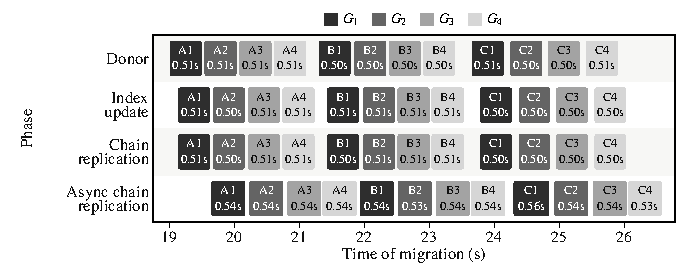
\includegraphics{experiments/crash_recovery/figures/HEALTHY.pdf}
  \end{subfigure}\hfill
  \begin{subfigure}[t]{2.40in}
    \hspace*{0.162in}\begin{minipage}{2.22in}\centering
      \caption{what the clients see over the same run}\label{fig:healthy-ycsb}
    \end{minipage}
    % (a) spends its top 0.154in on the group legend, so (b) is drawn that much shorter and
    % pushed down by the same amount: the two plot frames then share a top and a bottom edge.
    \par\centering\vspace*{0.154in}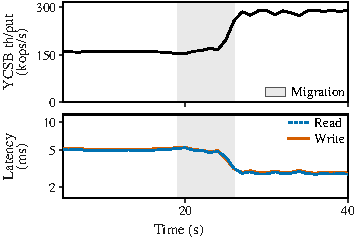
\includegraphics{experiments/crash_recovery/figures/healthy_ycsb.pdf}
  \end{subfigure}
  \caption{The no-fault migration.}
  \label{fig:healthy}
\end{figure*}

\paragraph{Timeouts.}
Failures are detected through timeouts or broken connections (Section~\ref{sec:fault-model}), so every wait that depends on another node has a timeout.
When the donor leader sends \texttt{RDMA\_DONE($G_i$)} and no \texttt{DURABLE} follows, it sends \texttt{QUERY\_STATE($G_i$)} to the recipient leader, which finds the new leader if the old one has gone.
It queries again whenever that \texttt{QUERY\_STATE($G_i$)} goes unanswered, and whenever no \texttt{DURABLE} follows a \texttt{TRANSFERRED} reply or a new transfer.
On the recipient side, a leader that asked for the data and never saw \texttt{RDMA\_DONE} asks once more.
A newly elected recipient leader gives the replicas one heartbeat interval to report their flags, and counts a silent replica as lacking the data.
Each of these actions is a query or a new transfer, both of which can be repeated safely, and every decision rests on committed log entries.
An early timeout costs one extra transfer at worst, and a late one only delays the recovery.

\iffalse
Fig.~\ref{fig:recipient_recovery} shows a recipient leader crash: B1 crashes after receiving $G_i$ but before replicating it, so the new leader B2 finds $G_i$ in flight without holding its data, obtains it again from the donor, and completes the migration.

\begin{figure}[t]
  \centering
  \begin{tikzpicture}[x={\columnwidth/252},y=-1pt,
    font=\fontsize{7.5}{9}\fontfamily{phv}\selectfont,
    >={Stealth[length=4pt,width=3.2pt]},
    lifeline/.style={draw=lifegray,line width=0.8pt},
    deadline/.style={draw=lifegray,line width=0.8pt,dash pattern=on 1pt off 2pt},
    shard/.style={draw=ink,line width=0.6pt,fill=white,rounded corners=1.5pt,
                  minimum width=24pt,minimum height=12pt,inner sep=0pt},
    leader/.style={shard,fill=ink,text=white,font=\fontsize{7.5}{9}\fontfamily{phv}\bfseries},
    msg/.style={->,draw=ink,line width=0.6pt},
    bulk/.style={->,draw=ink,line width=1.8pt,>={Stealth[length=5pt,width=5pt]}},
    notify/.style={->,draw=ink,line width=0.6pt,dash pattern=on 2.2pt off 1.4pt},
    crash/.style={draw=ink,line width=1.6pt,line cap=round},
    lbl/.style={inner sep=1pt,text=ink},
    phase/.style={rounded corners=2pt},
    phaselbl/.style={anchor=north west,inner sep=1.5pt,outer sep=0pt,
                     font=\fontsize{7.5}{9}\fontfamily{phv}\bfseries},
  ]
  \definecolor{ink}{RGB}{34,34,34}
  \definecolor{lifegray}{RGB}{165,165,165}
  \definecolor{llfill}{gray}{0.93}
  \definecolor{irfill}{gray}{0.86}
  \def\Gi{\textit{G}\textsubscript{\textit{i}}}
  \def\us{{\fontencoding{T1}\selectfont\_}}%
  \def\rstep#1{\tikz[baseline={([yshift=-2.7pt]s.center)}]\node[circle,fill=ink,text=white,inner sep=0pt,minimum size=9.6pt,text height=5.1pt,text depth=0.7pt,font=\fontsize{7.2}{7.2}\fontfamily{phv}\bfseries\selectfont](s){#1};}
  \def\xmark{\tikz[baseline=-2.7pt]{\draw[crash] (-3pt,-3pt) -- (3pt,3pt); \draw[crash] (-3pt,3pt) -- (3pt,-3pt);}}

  \def\Ah{26}
  \def\Bo{100} \def\Bt{163} \def\Bh{226}
  \def\crashy{97}
  \def\bottom{302}

  \fill[phase,llfill] (0,50) rectangle (252,106);
  \fill[phase,irfill] (0,111) rectangle (252,282);

  \foreach \x in {\Ah,\Bt,\Bh} \draw[lifeline] (\x,33) -- (\x,\bottom);
  \draw[lifeline] (\Bo,33) -- (\Bo,\crashy);
  \draw[deadline] (\Bo,\crashy) -- (\Bo,\bottom);

  \node[font=\fontsize{7.5}{9}\fontfamily{phv}\bfseries,anchor=base] at (\Ah,6) {Donor};
  \node[font=\fontsize{7.5}{9}\fontfamily{phv}\bfseries,anchor=base] at (\Bt,6) {Recipient shard group};
  \draw[ink,line width=0.5pt] (\Ah-14,15) -- ++(0,-3) -- (\Ah+14,12) -- ++(0,3);
  \draw[ink,line width=0.5pt] (\Bo-14,15) -- ++(0,-3) -- (\Bh+12,12) -- ++(0,3);
  \node[leader] at (\Ah,27) {A3};
  \node[leader] at (\Bo,27) {B1};
  \node[shard]  at (\Bt,27) {B2};
  \node[shard]  at (\Bh,27) {B3};
  \node[lbl,fill=white,font=\fontsize{7}{8}\fontfamily{phv}\itshape] at (\Ah,41) {leader};
  \node[lbl,fill=white,font=\fontsize{7}{8}\fontfamily{phv}\itshape] at (\Bo,41) {leader};

  \node[phaselbl,fill=llfill] at (2,52) {Before the crash};
  \draw[bulk] (\Ah,76) -- node[lbl,above=2pt,fill=llfill] {transfer} (\Bo,76);
  \draw[msg]  (\Ah,89) -- node[lbl,above=2pt,fill=llfill] {done}     (\Bo,89);
  \draw[crash] (\Bo-4.2,\crashy-4) -- (\Bo+4.2,\crashy+4);
  \draw[crash] (\Bo-4.2,\crashy+4) -- (\Bo+4.2,\crashy-4);
  \node[lbl,right=5pt,fill=llfill,font=\fontsize{7.5}{9}\fontfamily{phv}\bfseries] at (\Bo,\crashy) {B1 crashes};

  \node[phaselbl,fill=irfill] at (2,113) {Recovery};
  \node[leader,minimum width=30pt] at (\Bt,126) {leader};
  \node[lbl,right=3pt,fill=irfill,anchor=west] at (\Bt+15,126) {\rstep{a}\hspace{2pt}elected};

  \draw[msg,rounded corners=2pt] (\Bt,141) -- ++(12,0) -- ++(0,9) -- (\Bt,150);
  \node[lbl,right=3pt,fill=irfill,align=left,anchor=west] at (\Bt+12,145.5)
    {\rstep{b}\hspace{2pt}\Gi{} in flight,\\\hspace{11.6pt}data missing};

  \draw[msg]  (\Bt,170) -- node[lbl,above=2pt,fill=irfill] {\rstep{c}\hspace{2pt}resend \Gi} (\Ah,170);
  \draw[msg]  (\Ah,183) -- node[lbl,above=2pt,fill=irfill] {prepare}  (\Bt,183);
  \draw[msg]  (\Bt,196) -- node[lbl,above=2pt,fill=irfill] {MRs}      (\Ah,196);
  \draw[bulk] (\Ah,211) -- node[lbl,above=2pt,fill=irfill] {\rstep{d}\hspace{2pt}transfer} (\Bt,211);
  \draw[msg]  (\Ah,224) -- node[lbl,above=2pt,fill=irfill] {done}     (\Bt,224);

  \draw[bulk] (\Bt,241) -- node[lbl,above=2pt,align=center,font=\fontsize{7.5}{8}\fontfamily{phv}\selectfont] {\rstep{e}\hspace{2pt}chain\\replication} (\Bh,241);
  \draw[msg]  (\Bh,254) -- node[lbl,above=2pt,fill=irfill] {ack (2/3)} (\Bt,254);
  \node[lbl,above=2pt,fill=irfill] at ({(\Bt+\Bh)/2},274) {\rstep{f}\hspace{2pt}TRANSFER\us DURABLE(\Gi)};
  \draw[notify] (\Bt,274) -- (\Bh,274);

  \node[lbl,above=2pt,fill=white] at ({(\Ah+\Bt)/2},297) {\rstep{g}\hspace{2pt}DONE(\Gi)};
  \draw[msg] (\Bt,297) -- (\Ah,297);

  \def\key#1{\tikz[baseline=-2.7pt]\draw[#1] (0pt,0pt) -- (16pt,0pt);\hspace{3pt}}
  \node[inner sep=0pt,anchor=base] at (126,318) {%
    \key{msg}RPC\hspace{11pt}%
    \key{notify}Log entry\hspace{11pt}%
    \key{bulk}RDMA write\hspace{11pt}%
    \xmark\hspace{3pt}Crash};
\end{tikzpicture}%

  \caption{Recovery of group $G_i$ after the recipient leader crashes.
  (a)~B2 is elected leader.
  (b)~Its log holds \texttt{TXN\_START($G_i$)} but not \texttt{TRANSFER\_DURABLE($G_i$)}, and B2 lacks the data.
  (c--d)~The donor resends $G_i$ to B2.
  (e)~B2 replicates it to B3, reaching a majority.
  (f)~B2 commits \texttt{TRANSFER\_DURABLE($G_i$)}.
  (g)~The donor commits \texttt{DONE($G_i$)}.}
  \label{fig:recipient_recovery}
\end{figure}
\fi

\subsection{Chain replication}
\label{sec:chain-replication}

The recipient leader replicates the data of $G_i$ to its followers with chain replication over RDMA, in parallel with its own index update of $G_i$ (Section~\ref{sec:index_updating}).
The leader orders the live replicas into a chain and writes the data to the first one.
Each replica that has received the data forwards it to its successor and signals it with a \texttt{CHAIN\_DONE} message~(step~\mstep{4}).
The chain is set up before the migration starts, off its critical path.
The recipient leader opens an RDMA connection to every follower and registers landing buffers on each of them.
The followers also connect to each other, so any replica can forward the data to any other.
Each transaction gets its own transaction ID and its own landing buffers on every replica, so the groups of concurrent donors never overwrite each other.

\paragraph{Transfer state.}
The leader learns the state of the transfer without extra messages.
Every replica piggybacks it on its replies to the leader's \texttt{AppendEntries} messages, reporting which landing buffers of $G_i$ it holds and whether its transferred flag is set.
One-sided RDMA writes do not notify the replica they write to.
A replica therefore sets its flag only when the message that follows the data arrives, \texttt{RDMA\_DONE} from the donor or \texttt{CHAIN\_DONE} from its predecessor.
The leader knows at any time how far the data has travelled down the chain.
It learns that a majority holds $G_i$ once $f$ followers have reported it, without waiting for the rest of the chain.
Replication to this majority is synchronous. The remaining replicas receive the data asynchronously from the ongoing chain.

\paragraph{Chain repair.}
Each replica in the chain keeps a timeout for its successor.
The timeout starts when the replica forwards $G_i$ to its successor, and stops when the successor acknowledges that it holds $G_i$.
If the timeout expires, the replica reports it to the leader in its next reply to the leader's \texttt{AppendEntries} messages.
The leader then moves the successor to the end of the chain.
It tells the closest replica before it that holds $G_i$ to forward the data to the next replica in the new order.
This is the leader itself if no follower before the moved replica holds $G_i$.
The data does not change during the transfer, so the forwarding replica sends the whole of $G_i$ again and needs no record of what it sent before.
A replica whose RDMA connection to its successor breaks reports it in the same way, without waiting for the timeout.
The leader moves that successor to the end of the chain as well.
A replica that crashed and rejoins reports a cleared flag, and the leader adds it at the end of the chain.

The leader counts a replica as holding $G_i$ only when that replica reports it, so a timeout never makes \texttt{TRANSFER\_DURABLE($G_i$)} commit early.
% A timeout that fires too early only moves a slow replica to the end of the chain, where it still receives the data.
